\documentclass[10pt]{article}
\usepackage{iclr2026_conference}
\iclrfinalcopy
\iclrconference{ICLR-style research and implementation proposal for PCS 5022 / PhD article planning}

\usepackage[utf8]{inputenc}
\usepackage[T1]{fontenc}
\usepackage{amsmath,amssymb,mathtools}
\usepackage{booktabs}
\usepackage{array}
\usepackage{longtable}
\usepackage{tabularx}
\usepackage{multirow}
\usepackage{enumitem}
\usepackage{microtype}
\usepackage{graphicx}
\usepackage{xcolor}
\usepackage{xurl}
\usepackage{hyperref}
\usepackage{url}
\usepackage{tikz}
\usepackage{listings}
\usepackage{fancyvrb}
\usetikzlibrary{arrows.meta,positioning,fit,calc,shapes.geometric}
\Urlmuskip=0mu plus 1mu
\emergencystretch=3em
\sloppy
\hypersetup{colorlinks=true, linkcolor=black, citecolor=blue, urlcolor=blue}

\newcolumntype{Y}{>{\raggedright\arraybackslash}X}
\newcolumntype{L}[1]{>{\raggedright\arraybackslash}p{#1}}
\newcommand{\method}{Utility-PEFT}
\newcommand{\x}{\mathbf{x}}
\newcommand{\z}{\mathbf{z}}
\newcommand{\W}{\mathbf{W}}
\newcommand{\R}{\mathbb{R}}
\newcommand{\D}{\mathcal{D}}
\newcommand{\Mcal}{\mathcal{M}}
\newcommand{\Acal}{\mathcal{A}}
\newcommand{\Lcal}{\mathcal{L}}
\newcommand{\Ccal}{\mathcal{C}}
\newcommand{\Ucal}{\mathcal{U}}
\newcommand{\Scal}{\mathcal{S}}
\newcommand{\Ecal}{\mathcal{E}}
\newcommand{\eps}{\varepsilon}

\definecolor{codegray}{RGB}{245,245,245}
\lstset{
  basicstyle=\ttfamily\footnotesize,
  backgroundcolor=\color{codegray},
  frame=single,
  breaklines=true,
  columns=fullflexible,
  keepspaces=true,
  showstringspaces=false
}

\title{\method: Learning the Counterfactual Value of Adaptation Modules for Time-Series Foundation Models}

\author{Renan \quad Julia Martins Frejat \quad Chi-Nan Pai \quad Artur Jord\~ao\\
University of S\~ao Paulo / Escola Polit\'ecnica \quad \textit{working author list placeholder}}

\begin{document}
\maketitle

\begin{abstract}
Time-series foundation models (TSFMs) can transfer across datasets and tasks, but the best parameter-efficient fine-tuning (PEFT) procedure is strongly target-dependent. Recent time-series-specific methods expose an important limitation of importing low-rank allocation heuristics from natural language processing: global, static, or irreversible capacity allocation can suppress locally useful temporal behavior. Time-PEFT addresses temporal and multichannel complexity with fixed frequency and channel adapters; TRACE selects LoRA modules through target-specific masking-based importance estimation; TS-PET allocates ranks using interaction-aware pruning; AT4TS performs target-specific fine-tuning search; and MixFT trains a library of adapters for inferred temporal subdomains. These methods improve adaptation, but none directly predicts the \emph{counterfactual downstream value} of activating a candidate adaptation operation on a previously unseen dataset or regime.

We propose \method, an amortized, budget-aware policy that estimates the expected query-set improvement of candidate adapter families, LoRA layer groups, and effective ranks before full adaptation. Given a small support episode, the policy combines time-series structure, frozen-model mismatch, and cheap gradient probes to predict the utility and interaction of candidate modules. It then selects a sparse configuration maximizing expected improvement minus parameter, memory, and compute costs. The primary implementation uses MOMENT-base, a finite adapter action space, support/query episodic training, and a learning-to-rank utility predictor. Evaluation spans the forecasting datasets used by Time-PEFT, held-out multivariate classification tasks, and EMG adaptation through NinaPro DB6, NinaPro DB3, and EMGBench. The proposal includes an implementation blueprint, controlled baselines, resource-matched protocols, ablations, falsification criteria, and a staged plan suitable for implementation by an autonomous coding agent in a GPU environment.
\end{abstract}

\section{Introduction}

Parameter-efficient fine-tuning adapts a frozen foundation model by training a small set of additional or selected parameters. LoRA represents a weight update as a low-rank product and is widely used because it reduces trainable parameters while preserving the pretrained backbone \citep{hu2022lora}. However, uniform ranks and manually selected insertion points can be suboptimal. AdaLoRA allocates rank through importance scores derived from singular triplets \citep{zhang2023adalora}; AutoLoRA uses meta-learning to select rank-one components \citep{zhang2024autolora}; FlexLoRA permits rank pruning and expansion under a global budget \citep{liu2026flexlora}; and CoTo uses stochastic adapter activation and cooperative-game analysis of marginal contribution \citep{zhuang2025coto}. These methods show that adaptation capacity is neither uniform nor equally useful across model components.

The mismatch is particularly acute for time series. Temporal patterns may be localized, nonstationary, multiscale, and distributed unevenly across channels. TRACE argues that global singular-value importance and irreversible early pruning can overlook local temporal events and later-useful components; it instead uses reversible gates and simulated masking to estimate target-specific LoRA module importance \citep{li2026trace}. Time-PEFT introduces dataset-level temporal complexity based on spectral entropy and multichannel complexity based on lagged transfer entropy, then augments LoRA with a frequency adapter and a channel adapter \citep{na2026timepeft}. TS-PET proposes interaction-aware rank allocation and a lightweight prediction head \citep{zheng2026tspet}. AT4TS automates selective fine-tuning through target-specific hyperparameter optimization \citep{tomar2025at4ts}, while MixFT discovers latent temporal subdomains and trains one LoRA module per inferred component \citep{lee2026mixft}.

These papers establish that \emph{time-series adaptation must be specialized}. They leave a sharper question open:

\begin{quote}
Can a model predict, from a small target episode, which adaptation operation will actually improve downstream performance and justify its computational cost, without running a new exhaustive search or target-specific pruning procedure?
\end{quote}

This question is different from estimating data complexity. Spectral entropy and transfer entropy describe the input distribution, but they do not directly measure whether the frozen model already represents that structure or whether activating a specific adapter will improve the target task. Similarly, gradient importance measured after repeated target-specific training does not provide an amortized decision rule transferable across datasets. We therefore formulate adaptation selection as \emph{counterfactual utility prediction}.

For an episode $e$ and adaptation action $a$, the utility is the normalized query-loss reduction obtained after adapting on the support set, minus a weighted resource cost. During meta-training, actions are evaluated on source datasets to construct utility labels. A learned policy then predicts utilities for unseen episodes using three evidence families: (i) time-series structure; (ii) mismatch between the frozen model and the target episode; and (iii) cheap gradient probes estimating the responsiveness of candidate modules. At deployment, the policy chooses the best action under a budget and only then performs adaptation.

\paragraph{Research goal.}
Develop and validate a transferable adaptation-value predictor that selects PEFT components for unseen time-series datasets, tasks, subjects, and sessions more accurately and cheaply than fixed configurations, complexity thresholds, target-specific search, or pruning-based allocation.

\paragraph{Main contributions proposed.}
\begin{enumerate}[leftmargin=*, itemsep=2pt, topsep=2pt]
    \item A distinction between \emph{data complexity} and \emph{adaptation utility}, formalizing the latter as the counterfactual value of a PEFT action under an explicit resource budget.
    \item A modular TSFM adaptation bank spanning the task head, LoRA layer groups and ranks, frequency adaptation, and channel adaptation.
    \item An amortized utility predictor using structural descriptors, frozen-model mismatch, and one-step gradient probes, with pairwise terms for adapter synergy and conflict.
    \item A cross-dataset episodic training and evaluation protocol that measures oracle regret, negative transfer, configuration-ranking quality, and adaptation cost.
    \item A staged implementation and experiment plan covering forecasting, generic multivariate classification, and longitudinal/cross-subject EMG adaptation.
\end{enumerate}

\section{Novelty boundary and related work}

\subsection{Time-series-specific PEFT}

Time-PEFT measures temporal complexity through normalized spectral entropy and multichannel complexity through lagged transfer entropy. These statistics serve as indicators of where its specialized frequency and channel adapters provide larger gains \citep{na2026timepeft}. The architecture, however, uses a fixed combination of LoRA, frequency, channel, and forecast-head modules with predefined LoRA layers and ranks. Its own results show that additional modules can be unnecessary on lower-complexity standard datasets. This motivates selection, but a rule such as ``high transfer entropy implies channel adapter'' would be only an incremental extension.

TRACE replaces AdaLoRA-style importance with Gated Dynamic Simulation Importance Calculation and reconstructs large forecasting heads \citep{li2026trace}. Its selection is reversible and target-specific, but requires importance estimation during adaptation on each target. TS-PET estimates synergistic rank interactions and uses stochastic approximation, but it remains a target-specific rank-allocation method \citep{zheng2026tspet}. MixFT routes contexts to adapters trained for discovered subdomains, whereas \method aims to compose an adaptation configuration for an unseen target rather than retrieve a previously trained subdomain expert \citep{lee2026mixft}. AT4TS is an important search baseline because it automates selective fine-tuning, but its optimization cost is paid again for each target domain \citep{tomar2025at4ts}.

\subsection{Automatic and meta-learned PEFT}

AdaLoRA, AutoLoRA, dEBORA, FlexLoRA, and LoRA-Drop address rank or module allocation using importance, meta-gradients, bilevel optimization, entropy, or pruning \citep{zhang2023adalora,zhang2024autolora,zangrando2025debora,liu2026flexlora,zhou2025loradrop}. Meta-Adapters and recent provable PEFT meta-learning prepare models for rapid low-dimensional adaptation across tasks \citep{bansal2022metaadapters,block2025provable}. These works motivate amortization across tasks, but do not predict the utility of heterogeneous time-series adapter families under a resource budget.

CoTo is particularly relevant because it quantifies adapter marginal contributions using a cooperative-game view \citep{zhuang2025coto}. \method differs in objective and deployment: CoTo improves training and post-hoc operations for a given target, whereas \method predicts target-episode-specific counterfactual gains before committing to full adaptation. The comparison nevertheless requires care, and a CoTo-style marginal-contribution estimator is included as a baseline or label-acceleration mechanism.

\subsection{Time-series foundation models and tasks}

MOMENT is the primary backbone because it is open, supports multiple downstream tasks, and is used by Time-PEFT and related TSFM adaptation work \citep{goswami2024moment}. UniTS is the secondary backbone because it unifies forecasting, classification, anomaly detection, and imputation across heterogeneous domains \citep{gao2024units}. Chronos, TimesFM, Tiny Time Mixers, Sundial, and other TSFMs provide additional context, but the first article should avoid an unnecessarily broad backbone matrix \citep{ansari2024chronos,das2024timesfm,ekambaram2024ttm,liu2025sundial}.

\subsection{EMG as a held-out adaptation domain}

EMGBench standardizes intersubject generalization and adaptation across nine electromyography datasets \citep{yang2024emgbench}. NinaPro DB6 contains repeated grasp sessions across five days and is therefore suitable for chronological session/day shifts \citep{palermo2017db6}. NinaPro DB3 contains transradial amputee participants and provides a clinically meaningful population shift \citep{atzori2015ninapro}. EMG is not the source of the method's novelty; it is a demanding held-out domain where temporal structure, channel relations, sensor placement, session drift, and user variation can make adaptation choices materially different.

\section{Problem formulation}

\subsection{Episodes, backbone, and adaptation actions}

Let $f_{\theta}$ be a pretrained TSFM with frozen parameters $\theta$. An adaptation episode is
\begin{equation}
 e = (\D_e^{\mathrm{sup}},\D_e^{\mathrm{qry}}),
\end{equation}
where the support set is available for fine-tuning and the query set is used only to measure the consequence of the adaptation action during meta-training or evaluation. The target deployment setting may be supervised few-shot, weakly supervised, or source-free; the primary implementation uses labeled few-shot support to isolate the adaptation-selection problem cleanly.

An action $a\in\Acal$ specifies a subset and configuration of adaptation modules. The minimum viable action space is
\begin{equation}
\Acal_{\mathrm{MVP}}=
\{\varnothing,H,H{+}L,H{+}L{+}F,H{+}L{+}C,H{+}L{+}F{+}C,H{+}\mathrm{FourierFT}\},
\end{equation}
where $H$ is the task head, $L$ is fixed-rank LoRA on predefined backbone projections, $F$ is a frequency adapter, and $C$ is a channel adapter. Full fine-tuning is an upper reference rather than a deployable controller action.

The extended action space factorizes an action as
\begin{equation}
 a=(S_a,G_a,r_a,b_a),
\end{equation}
where $S_a$ is the adapter-family subset, $G_a$ is the selected layer group, $r_a$ is the effective LoRA rank, and $b_a$ is the update budget such as epochs or steps.

\subsection{Counterfactual adaptation utility}

Let $\ell_0(e)$ denote the query loss of the frozen or head-only reference, and let $\ell_a(e)$ denote the query loss after adapting action $a$ on $\D_e^{\mathrm{sup}}$. Define normalized performance gain
\begin{equation}
\Delta(e,a)=\frac{\ell_0(e)-\ell_a(e)}{|\ell_0(e)|+\eps}.
\end{equation}

Let $c_p$, $c_f$, $c_m$, and $c_t$ denote normalized active-parameter, backward-FLOP, peak-memory, and wall-clock costs. The action utility is
\begin{equation}
U(e,a)=\Delta(e,a)
-\lambda_p c_p(a)
-\lambda_f c_f(a)
-\lambda_m c_m(a)
-\lambda_t c_t(a).
\label{eq:utility}
\end{equation}

The nondeployable oracle action is
\begin{equation}
a_e^{\star}=\arg\max_{a\in\Acal}U(e,a).
\end{equation}

The goal is to learn $\widehat U_{\psi}(e,a)$ such that
\begin{equation}
\widehat a_e=\arg\max_{a\in\Acal:\,\Ccal(a)\le B} \widehat U_{\psi}(e,a)
\end{equation}
achieves low oracle regret on datasets and regimes excluded from policy training.

\subsection{Why utility is different from complexity}

Time-series complexity is a property of the episode. Adaptation utility is a property of the tuple $(e,a,f_{\theta})$. Two episodes can have similar spectral and transfer entropy but different utility because the frozen model represents one well and the other poorly. Likewise, a highly multichannel dataset need not benefit from a channel adapter if the backbone already models the relevant dependence. This motivates conditioning on the frozen model and candidate action rather than routing from raw complexity thresholds alone.

\section{Proposed method: \method}

\subsection{System overview}

\begin{figure}[t]
\centering
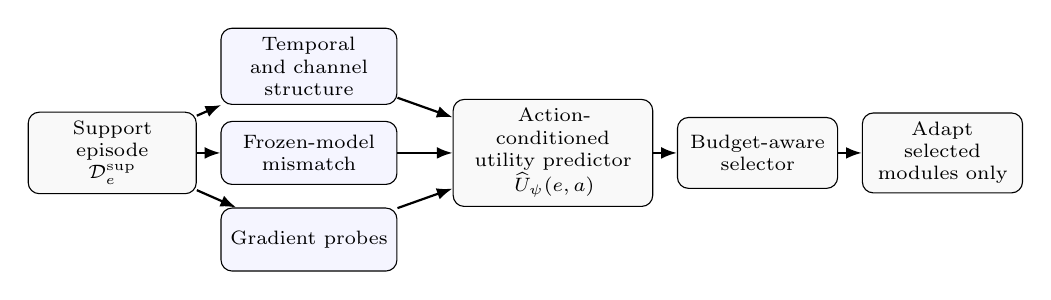
\begin{tikzpicture}[
  node distance=4mm and 3mm,
  every node/.style={font=\scriptsize},
  box/.style={draw, rounded corners, align=center, minimum height=9mm, text width=19mm, fill=gray!5},
  smallbox/.style={draw, rounded corners, align=center, minimum height=8mm, text width=20mm, fill=blue!4},
  arrow/.style={-{Latex[length=2mm]}, thick}
]
\node[box] (episode) {Support episode\\$\D_e^{\mathrm{sup}}$};
\node[smallbox, right=of episode, yshift=11mm] (struct) {Temporal and channel structure};
\node[smallbox, right=of episode] (shift) {Frozen-model mismatch};
\node[smallbox, right=of episode, yshift=-11mm] (grad) {Gradient probes};
\node[box, right=7mm of shift, text width=23mm] (predictor) {Action-conditioned\\utility predictor\\$\widehat U_\psi(e,a)$};
\node[box, right=of predictor, text width=18mm] (selector) {Budget-aware\\selector};
\node[box, right=of selector, text width=18mm] (adapt) {Adapt selected\\modules only};
\draw[arrow] (episode) -- (struct);
\draw[arrow] (episode) -- (shift);
\draw[arrow] (episode) -- (grad);
\draw[arrow] (struct) -- (predictor);
\draw[arrow] (shift) -- (predictor);
\draw[arrow] (grad) -- (predictor);
\draw[arrow] (predictor) -- (selector);
\draw[arrow] (selector) -- (adapt);
\end{tikzpicture}
\caption{\method{} predicts the value of candidate adaptation operations before full fine-tuning. Transfer entropy is an optional structural feature, not the routing rule or source of novelty.}
\label{fig:overview}
\end{figure}

\subsection{Modular adapter bank}

The first implementation uses a shared modular bank:
\begin{equation}
\Mcal=\{H,L,F,C\}.
\end{equation}

\paragraph{Head $H$.} A task-specific linear or shallow prediction head. It is always available and may be trained alone.

\paragraph{LoRA $L$.} For a selected weight matrix $\W_{\ell}$,
\begin{equation}
\W_{\ell}'=\W_{\ell}+\alpha_{\ell}\sum_{j=1}^{R_{\max}}g_{\ell j}b_{\ell j}a_{\ell j}^{\top}.
\end{equation}
The MVP fixes the target projections and $r=8$. The extended implementation uses nested rank-one units, enabling effective ranks $r\in\{2,4,8,16\}$ without SVD pruning.

\paragraph{Frequency adapter $F$.} A Time-PEFT-compatible module that transforms backbone embeddings along the patch/time axis, retains dominant or learned frequency components, reconstructs a filtered representation, and combines it with the original representation \citep{na2026timepeft}. The first reproduction should match Time-PEFT's top-$k$ implementation before introducing learned or localized alternatives.

\paragraph{Channel adapter $C$.} A shared down-projection and channel-specific up-projection module inspired by Time-PEFT, adapted to both forecasting and classification heads \citep{na2026timepeft}. For very high channel counts, grouped or low-rank channel projections are required to control parameter growth.

\subsection{Evidence available to the utility predictor}

The episode representation is
\begin{equation}
\z_e=[\z_e^{\mathrm{struct}}\Vert\z_e^{\mathrm{mismatch}}\Vert\z_e^{\mathrm{grad}}\Vert\z_e^{\mathrm{meta}}].
\end{equation}

\paragraph{Time-series structure.} Candidate descriptors include normalized spectral entropy, spectral concentration, autocorrelation decay, trend strength, multiscale energy, transient/change-point density, channel count, sampling metadata, transfer-entropy summaries, and cheap alternatives such as lagged correlation or mutual information. Transfer entropy should be treated as an ablated feature because its $O(C^2L)$ cost can become prohibitive for dense EMG.

\paragraph{Frozen-model mismatch.} Candidate signals include frozen support loss, representation distance to source prototypes, masked-reconstruction loss, prediction entropy, calibration, feature covariance shift, and disagreement under time-series augmentations. These features distinguish data complexity from whether the pretrained model already handles it.

\paragraph{Gradient probes.} Initialize all candidate modules with zero-impact parameterization, perform one support backward pass, and record group-level statistics without applying an update. For module $m$:
\begin{equation}
q_m(e)=\left[\|g_m\|_2,\;\|g_m\|_\infty,\;\mathrm{Var}(g_m),\;\mathrm{SNR}(g_m),\;\cos(g_m,g_H)\right],
\end{equation}
where $g_m=\nabla_{\phi_m}\Lcal_{\mathrm{sup}}$. The first-order predicted gain $\eta\|g_m\|_2^2$ is included as a feature, not assumed to be an exact utility estimate.

\paragraph{Episode metadata.} Support size, number of channels, lookback length, horizon, task type, and backbone identity are encoded explicitly. Dataset names are never provided to the controller in held-out-dataset evaluation.

\subsection{Action-conditioned utility predictor}

Each action has an embedding $v_a$ describing its active module families, layer groups, rank, and budget. The predictor receives $(\z_e,v_a)$ and outputs a mean and uncertainty:
\begin{equation}
(\mu_{ea},\log\sigma^2_{ea})=h_{\psi}([\z_e\Vert v_a]).
\end{equation}

A heteroscedastic regression loss is combined with pairwise ranking:
\begin{align}
\Lcal_{\mathrm{reg}}&=\sum_{e,a}\frac{(U(e,a)-\mu_{ea})^2}{2\sigma^2_{ea}}+\frac{1}{2}\log\sigma^2_{ea},\\
\Lcal_{\mathrm{rank}}&=\sum_{e,a^+,a^-}\max\{0,\gamma-\mu_{ea^+}+\mu_{ea^-}\},\\
\Lcal_{\mathrm{utility}}&=\Lcal_{\mathrm{reg}}+\beta\Lcal_{\mathrm{rank}}.
\end{align}

Ranking is more important than exact calibration because deployment requires choosing a good action. Utility uncertainty supports conservative selection: if the expected gain is smaller than its uncertainty-adjusted margin, the policy can choose the no-op or head-only action.

\subsection{Interaction-aware utility}

Adapter effects need not be additive. Time-PEFT reports synergy between LoRA, frequency, and channel modules, while TS-PET and CoTo motivate interaction-aware importance \citep{na2026timepeft,zheng2026tspet,zhuang2025coto}. A factorized alternative predicts
\begin{equation}
\widehat U(e,S)=\sum_{m\in S}\widehat u_m(e)+\sum_{m<n;\,m,n\in S}\widehat u_{mn}(e)-\lambda\Ccal(S).
\end{equation}
The MVP can directly enumerate seven actions. The factorized formulation becomes useful when layer groups and ranks expand the action space.

\subsection{Budget-aware selection}

For the MVP, enumerate all actions satisfying the active-parameter or backward-FLOP budget. For the extended action space, use beam search or a small binary integer program. The selector should support three deployment policies:
\begin{enumerate}[leftmargin=*, itemsep=1pt]
    \item \textbf{Accuracy-first}: maximize predicted gain with a soft cost penalty.
    \item \textbf{Hard budget}: maximize predicted gain subject to parameter, memory, or latency constraints.
    \item \textbf{Conservative}: adapt only when a lower confidence bound on utility is positive.
\end{enumerate}

\subsection{Constructing counterfactual utility labels}

Exact utility labels require adapting each candidate action, which is expensive but feasible for a small action set and moderate backbone. Labels are generated offline and cached. To scale beyond the MVP:
\begin{enumerate}[leftmargin=*, itemsep=1pt]
    \item use low-fidelity actions with fewer steps or smaller support subsets;
    \item apply successive halving to remove clearly inferior actions;
    \item exploit nested LoRA ranks so one maximum-rank run can yield partial-rank evaluations;
    \item warm-start compatible action supersets;
    \item use CoTo/TRACE-style masking estimates as auxiliary targets, never as the sole ground truth;
    \item retain exact full-budget labels for a stratified subset to calibrate low-fidelity bias.
\end{enumerate}

\subsection{Deployment settings}

\paragraph{Primary: labeled few-shot adaptation.} A small labeled support set is available, as in EMGBench adaptation protocols. This is the cleanest setting for validating utility selection.

\paragraph{Secondary: unlabeled/source-free adaptation.} Replace supervised support loss with masked reconstruction, consistency, entropy, or pseudo-label losses. The controller is either retrained for this objective or receives the objective type as part of the action. This extension should follow after the primary claim is established.

\paragraph{Online session adaptation.} For NinaPro DB6, recompute episode evidence at each new session and decide whether to preserve, reset, or replace the adapter state. This is a deployment extension, not required for the first complete result.

\section{Implementation strategy}

\subsection{Staged scope}

\begin{table}[t]
\centering
\caption{Implementation stages. Each stage should produce a testable artifact before expanding the action space.}
\label{tab:stages}
\begin{tabularx}{\textwidth}{L{0.12\textwidth}YY}
\toprule
Stage & Scope & Completion criterion \\
\midrule
0 & Reproduce MOMENT, LoRA, FourierFT, and Time-PEFT on a small subset & Results within reported variability or documented implementation discrepancy \\
1 & Build episode API, adapter bank, exact action evaluator, and cache & Deterministic utility table for at least three datasets \\
2 & Train utility predictor on structural, mismatch, and gradient evidence & Utility ranking exceeds complexity-only and random baselines \\
3 & Leave-one-dataset-out forecasting evaluation & Low oracle regret and favorable accuracy-cost frontier on unseen datasets \\
4 & Extend to MOMENT classification and EMGBench/NinaPro & Policy transfers across task and domain boundaries \\
5 & Add rank/layer factorization and secondary UniTS backbone & Gains survive larger action space and architecture change \\
6 & Optional source-free/online TTT extension & Stable adaptation without target-label leakage \\
\bottomrule
\end{tabularx}
\end{table}

\subsection{Recommended repository layout}

\begin{lstlisting}
utility-peft/
  configs/
    backbone/          # moment_base.yaml, units.yaml
    dataset/           # forecasting and EMG protocols
    action_space/      # mvp.yaml, extended.yaml
    experiment/        # reproduction, oracle_map, meta_train, heldout_eval
  src/utility_peft/
    backbones/         # unified encode/predict interface
    adapters/          # head, LoRA bank, frequency, channel, FourierFT
    episodes/          # support/query sampling and leakage checks
    descriptors/       # structural and mismatch features
    probes/            # gradient-hook statistics
    utility/           # action evaluator, cost model, cache schema
    controller/        # action encoder, utility predictor, selector
    training/          # adapter, label-generation, meta-training loops
    metrics/           # task, cost, regret, ranking, calibration
  scripts/
    reproduce_time_peft.py
    generate_utility_table.py
    train_utility_predictor.py
    evaluate_heldout.py
  tests/
    test_no_target_leakage.py
    test_zero_impact_adapters.py
    test_action_budget.py
    test_episode_chronology.py
  Makefile
  pyproject.toml
  README.md
\end{lstlisting}

\subsection{Core software interfaces}

\paragraph{Backbone adapter.} Every backbone wrapper should expose:
\begin{lstlisting}
encode(x, mask=None) -> embeddings
predict(x, task_spec) -> predictions
adapter_targets() -> named parameter groups
source_statistics() -> optional representation prototypes
\end{lstlisting}

\paragraph{Action specification.}
\begin{lstlisting}
ActionSpec(
  modules={"head", "lora", "frequency", "channel"},
  layer_group="last_half",
  rank=8,
  update_steps=100,
  budget={"max_trainable_pct": 4.0}
)
\end{lstlisting}

\paragraph{Episode specification.}
\begin{lstlisting}
Episode(
  support_x, support_y,
  query_x, query_y,
  task_type, dataset_family,
  subject_id=None, session_id=None,
  chronology_metadata=None
)
\end{lstlisting}

\paragraph{Utility record.}
\begin{lstlisting}
UtilityRecord(
  episode_id, action_id, seed,
  frozen_loss, adapted_loss,
  trainable_params, backward_flops,
  peak_memory_mb, wall_time_s,
  utility, descriptors, gradient_probes
)
\end{lstlisting}

\subsection{Reproducibility and engineering requirements}

\begin{enumerate}[leftmargin=*, itemsep=2pt]
    \item Pin exact model checkpoints, dataset versions, package commits, and preprocessing hashes.
    \item Store every split manifest and verify that target query labels never influence action selection.
    \item Use deterministic episode IDs and cache all action evaluations in Parquet or SQLite.
    \item Separate \emph{stored parameters} from \emph{active trainable parameters}; report both.
    \item Log measured GPU memory and wall-clock time rather than relying only on analytical counts.
    \item Add smoke tests with a tiny backbone and synthetic time series before GPU-scale runs.
    \item Implement resume-safe utility-table generation because this is the most expensive phase.
    \item Use Hydra or an equivalent configuration system so every table row can be regenerated from a committed config.
\end{enumerate}

\section{Experimental design}

\subsection{Backbones}

\paragraph{Primary backbone: MOMENT-base.} MOMENT provides open checkpoints and supports forecasting and classification \citep{goswami2024moment}. It also yields the cleanest comparison with Time-PEFT and TRACE.

\paragraph{Secondary backbone: UniTS.} UniTS is used only after the method is stable on MOMENT, testing whether the controller overfits one architecture \citep{gao2024units}.

\subsection{Datasets}

\paragraph{Forecasting reproduction and meta-training pool.}
Use the Time-PEFT suite:
\begin{itemize}[leftmargin=*, itemsep=1pt]
    \item complex/chaotic: Lorenz, CellCycle, DoublePendulum, Hopfield, LorenzCoupled;
    \item medical: ECGCA115 and ECGCA515;
    \item standard: ETTh1, ETTh2, ETTm1, ETTm2, Weather, Exchange.
\end{itemize}
The initial protocol follows lookback $96$ and horizons $\{96,192,336\}$ for comparability, with model-specific exceptions documented \citep{na2026timepeft}.

\paragraph{Generic multivariate classification.}
Select a stratified subset of the UEA multivariate archive spanning human motion, physiological signals, industrial sensors, and different channel counts \citep{bagnall2018uea}. The selection should be frozen before results are inspected. Candidate datasets include BasicMotions, CharacterTrajectories, Epilepsy, FingerMovements, Handwriting, MotorImagery, NATOPS, and SelfRegulationSCP1.

\paragraph{EMG.}
\begin{itemize}[leftmargin=*, itemsep=1pt]
    \item \textbf{NinaPro DB6}: cross-session and cross-day grasp recognition \citep{palermo2017db6}.
    \item \textbf{EMGBench}: official intersubject and adaptation protocols across nine datasets \citep{yang2024emgbench}.
    \item \textbf{NinaPro DB3}: leave-one-subject-out or held-out clinical population experiment with transradial amputees \citep{atzori2015ninapro}.
\end{itemize}

\subsection{Experiment E0: reproduction and adapter parity}

Reproduce the frozen, head-only, full fine-tuning, LoRA, FourierFT, ChannelMixing, and Time-PEFT results on a manageable subset: Lorenz, ECGCA115, ETTh1, and Weather. Verify adapter placement, parameter counts, and head architecture before generating utility labels. TRACE and TS-PET reproductions may begin from official code or carefully isolated subcomponents if full code is unavailable.

\subsection{Experiment E1: oracle adaptation map}

Evaluate every MVP action on source-dataset episodes. The objectives are:
\begin{enumerate}[leftmargin=*, itemsep=1pt]
    \item quantify how often the oracle action differs across datasets, horizons, and local regimes;
    \item measure the regret of one globally fixed configuration;
    \item determine whether Time-PEFT's two complexity scalars alone predict the oracle action;
    \item test whether the action ordering is stable across seeds and support sizes.
\end{enumerate}

This experiment can falsify the project early. If one fixed action is nearly always optimal after cost matching, a learned selector is unnecessary.

\subsection{Experiment E2: utility prediction on held-out forecasting datasets}

Use leave-one-dataset-out meta-evaluation. For each held-out dataset:
\begin{enumerate}[leftmargin=*, itemsep=1pt]
    \item train the utility predictor on all other datasets;
    \item expose only the held-out support episode and action metadata;
    \item select an action without target query labels;
    \item adapt on support and evaluate on the official test/query partition;
    \item compare with the target oracle, best source-fixed action, and target-specific search.
\end{enumerate}

A stronger leave-one-family-out protocol holds out all chaotic, all medical, or all standard datasets.

\subsection{Experiment E3: evidence ablation}

Train identical predictors with:
\begin{enumerate}[leftmargin=*, itemsep=1pt]
    \item Time-PEFT complexity scalars only;
    \item structural descriptors without transfer entropy;
    \item frozen-model mismatch only;
    \item gradient probes only;
    \item structure + mismatch;
    \item structure + gradient;
    \item mismatch + gradient;
    \item all evidence.
\end{enumerate}

This directly establishes whether the novelty comes from utility-oriented model evidence rather than reusing transfer entropy.

\subsection{Experiment E4: cross-task transfer to classification}

Meta-train the policy on forecasting only, then test zero-shot policy transfer to classification. Compare with a policy meta-trained on mixed forecasting and classification episodes. This separates general adaptation-value learning from forecasting-specific heuristics.

\subsection{Experiment E5: NinaPro DB6 chronological adaptation}

Use subject-disjoint and chronological splits. Two proposed tracks are:

\paragraph{Few-shot session adaptation.} Train the backbone/controller without the target subject. Use a small labeled calibration subset from the first target session or day, select an action, and evaluate on later sessions chronologically. Report support fractions such as $1\%$, $5\%$, and $20\%$ where feasible.

\paragraph{Rolling session adaptation.} At session $s$, the controller uses only data from sessions $\le s$ and predicts the action for session $s+1$. Compare reset, persistent, and reselected adapters. No future session statistics may be used.

Key analysis: whether channel-heavy actions are selected after electrode re-donning, frequency-related actions under fatigue-like drift, and no-op/head-only actions when the frozen model remains adequate. These interpretations are hypotheses, not hard-coded rules.

\subsection{Experiment E6: EMGBench and NinaPro DB3}

Follow official EMGBench intersubject and adaptation splits, preserving its preprocessing and evaluation protocol \citep{yang2024emgbench}. Hold out entire EMG datasets from controller training where possible. NinaPro DB3 is a dedicated transfer test: compare a controller trained on non-EMG time series, on intact-subject EMG, and on other amputee subjects.

\subsection{Experiment E7: extended rank and layer action space}

After the MVP succeeds, expand $G_a$ and $r_a$:
\begin{equation}
G_a\in\{\text{last block},\text{last half},\text{all blocks}\},\qquad
r_a\in\{2,4,8,16\}.
\end{equation}
Compare direct action enumeration, factorized module/pair utility, AutoLoRA, AdaLoRA, dEBORA, FlexLoRA, TRACE, and TS-PET. This is the experiment most directly related to the professor's questions about rank and layer selection.

\section{Baselines and fair comparison}

\begin{longtable}{L{0.20\textwidth}L{0.27\textwidth}L{0.43\textwidth}}
\caption{Baseline families and their role.}\label{tab:baselines}\\
\toprule
Baseline & Selection mechanism & Purpose \\
\midrule
\endfirsthead
\toprule
Baseline & Selection mechanism & Purpose \\
\midrule
\endhead
Frozen / zero-shot & None & Establish adaptation need. \\
Head-only & Fixed minimal update & Strong low-cost reference. \\
Full fine-tuning & All parameters & High-cost performance reference. \\
Fixed LoRA & Fixed layers and rank & Generic PEFT baseline. \\
FourierFT & Learned sparse Fourier coefficients & Frequency-domain generic PEFT baseline \citep{gao2024fourierft}. \\
Time-PEFT & Fixed LoRA + frequency + channel adapters & Direct time-series-specialized baseline \citep{na2026timepeft}. \\
AdaLoRA & SVD-based adaptive budget allocation & Global adaptive-rank comparator \citep{zhang2023adalora}. \\
AutoLoRA & Meta-learned rank-one selection & Closest meta-rank comparator \citep{zhang2024autolora}. \\
dEBORA / FlexLoRA & Bilevel or entropy-guided rank allocation & Modern adaptive-rank controls \citep{zangrando2025debora,liu2026flexlora}. \\
TRACE & Target-specific masking-based LoRA module importance & Reversible target-specific selection \citep{li2026trace}. \\
TS-PET & Interaction-aware pruned LoRA & Rank-interaction comparator \citep{zheng2026tspet}. \\
AT4TS & Target-specific HPO / selective tuning & Search-cost comparator \citep{tomar2025at4ts}. \\
MixFT & Subdomain discovery + adapter library & Regime-routing comparator \citep{lee2026mixft}. \\
CoTo & Stochastic adapter activation + marginal contribution & Training robustness and utility-estimation comparator \citep{zhuang2025coto}. \\
Complexity threshold router & Hand-coded Time-PEFT statistics & Tests whether learning utility is needed. \\
Random budget-matched action & Random feasible action & Detects action-space or regularization artifacts. \\
Best source-fixed action & One action selected on source validation & Primary fixed-policy baseline. \\
Target oracle & Exhaustive target query selection & Nondeployable upper reference and regret denominator. \\
\bottomrule
\end{longtable}

Every comparison must match or explicitly report the same backbone and checkpoint, support size, label and validation access, optimizer and update steps, active-parameter budget, and measured compute budget.
Methods using a target validation set, such as HPO or target-specific importance selection, should be reported in a separate information-access tier from amortized zero-search selection.

\section{Metrics and statistical analysis}

\subsection{Task metrics}

Forecasting uses MSE, MAE, and optionally MASE or sMAPE when scale comparability matters. Classification uses accuracy, macro-F1, balanced accuracy, and expected calibration error. Results are reported per dataset, subject/session, and task family rather than only as a grand average.

\subsection{Selection metrics}

\paragraph{Oracle regret.}
\begin{equation}
R_{\mathrm{oracle}}(e)=U(e,a_e^{\star})-U(e,\widehat a_e).
\end{equation}

\paragraph{Ranking quality.} Spearman correlation and NDCG between predicted and observed action utilities; top-1 and top-$k$ action accuracy.

\paragraph{Negative adaptation rate.}
\begin{equation}
\mathrm{NAR}=\frac{1}{N}\sum_e\mathbb{I}[\ell_{\widehat a_e}(e)>\ell_0(e)].
\end{equation}

\paragraph{Efficiency.} Active trainable parameters, stored adapter parameters, backward FLOPs, peak GPU memory, selection overhead, and adaptation wall time.

\paragraph{Pareto analysis.} Compare methods on performance versus active parameters, performance versus backward FLOPs, and performance versus wall time.

\subsection{Uncertainty and tests}

Use at least three adaptation seeds for exploratory experiments and five for final key tables. For multiple datasets, report paired bootstrap confidence intervals and Wilcoxon signed-rank tests over dataset/horizon or subject/session units, with Holm correction. Effect sizes should accompany $p$-values. Utility-predictor calibration is measured by reliability diagrams or interval coverage.

\section{Ablations and falsification criteria}

\subsection{Essential ablations}

\begin{enumerate}[leftmargin=*, itemsep=2pt]
    \item Complexity-only versus utility-oriented evidence.
    \item With and without transfer entropy; scalar TE versus lag-resolved graph summaries.
    \item With and without frozen-model mismatch features.
    \item With and without gradient probes.
    \item Individual module scores versus pairwise interaction terms.
    \item Exact utility labels versus low-fidelity/successive-halving labels.
    \item Regression only versus ranking only versus combined objective.
    \item Fixed action cost weights versus hard budgets and budget-conditioned controller.
    \item Dataset-level, session-level, and local-window episodes.
    \item Forecasting-only versus mixed-task meta-training.
    \item MOMENT-only versus MOMENT-to-UniTS transfer.
\end{enumerate}

\subsection{Falsification criteria}

The central hypothesis is weakened or rejected if:
\begin{enumerate}[leftmargin=*, itemsep=2pt]
    \item one globally fixed action matches \method on held-out datasets after cost matching;
    \item a two-threshold complexity router matches the learned utility predictor;
    \item gradient or mismatch evidence does not improve action ranking beyond Time-PEFT statistics;
    \item utility gains vanish when target-validation access and compute are matched;
    \item the policy collapses to nearly the same action for all targets;
    \item low oracle regret occurs only on datasets used to meta-train the controller;
    \item improvements appear only on EMG and do not reproduce on non-biomedical tasks;
    \item policy-inference overhead offsets the saved adaptation cost;
    \item utility labels are too unstable across seeds to support reliable ranking.
\end{enumerate}

\section{Expected results and interpretation}

The expected result is not universal dominance on every dataset. Static Time-PEFT may remain best on homogeneous high-complexity forecasting datasets, and head-only or LoRA may remain sufficient on standard datasets. The proposed method should be strongest where adaptation needs vary across datasets, horizons, tasks, subjects, or sessions.

A successful result pattern would show:
\begin{enumerate}[leftmargin=*, itemsep=2pt]
    \item lower oracle regret than complexity thresholds and best source-fixed policies on held-out datasets;
    \item comparable or better forecasting/classification performance with fewer active parameters than always-on Time-PEFT;
    \item lower search cost than AT4TS, TRACE, or exhaustive target validation;
    \item meaningful action variation rather than indiscriminate activation of all modules;
    \item transfer from forecasting meta-training to classification and EMG;
    \item reduced negative adaptation on NinaPro sessions where large updates are harmful.
\end{enumerate}

The most important scientific finding would be that target structure alone is insufficient: adaptation value becomes predictable only when structural descriptors are combined with evidence about the frozen model and the local optimization geometry.

\section{Risks and contingency plan}

\paragraph{Combinatorial action cost.} Begin with seven actions and exact labels. Expand only after utility ranking works. Use low-fidelity evaluation and factorization for larger spaces.

\paragraph{Utility labels are noisy.} Average over seeds, use ranking losses, model uncertainty, and treat near-ties as equivalent rather than forcing arbitrary labels.

\paragraph{Transfer entropy is expensive or unstable.} Treat it as optional. Compare lagged correlation, mutual information, PCA/grouped TE, and learned channel-graph summaries. The paper's novelty does not depend on TE.

\paragraph{Task mismatch.} Separate task-specific heads and normalize utilities. Evaluate cross-task transfer explicitly rather than assuming one policy works unchanged.

\paragraph{Backbone integration differences.} Freeze the primary claim on MOMENT before extending to UniTS. Document exact adapter targets per architecture.

\paragraph{No benefit over fixed policies.} The oracle-map experiment is an early stop. A negative result can still support a useful article if it shows that adaptation complexity does not justify a controller under realistic budgets, but the full implementation should not proceed blindly.

\section{Resource plan and milestones}

\begin{table}[h]
\centering
\caption{Indicative execution plan. Duration depends on official-code availability and GPU throughput.}
\begin{tabularx}{\textwidth}{L{0.12\textwidth}YY}
\toprule
Milestone & Deliverable & Main compute \\
\midrule
M1 & Reproduction report and tested adapter interfaces & Single GPU, small dataset subset \\
M2 & Exact MVP utility table and oracle-map analysis & Parallel action jobs on one or more GPUs \\
M3 & Utility predictor and held-out forecasting results & Light controller training + cached adaptations \\
M4 & UEA classification and cross-task transfer & Moderate GPU usage \\
M5 & NinaPro DB6 / EMGBench experiments & Data preprocessing + moderate fine-tuning \\
M6 & Extended rank/layer space and UniTS validation & Highest compute; run only after MVP success \\
M7 & Source-free/online extension and final paper & Optional second-stage study \\
\bottomrule
\end{tabularx}
\end{table}

The expensive artifact is the utility table, not the controller. Action evaluations should be embarrassingly parallel and resume-safe. A first credible paper can be completed with MOMENT-base, the MVP action space, forecasting leave-one-dataset-out evaluation, one classification suite, and NinaPro DB6; the extended architecture matrix is not required for the initial contribution.

\section{Relevance to assistive technology}

Patient-specific assistive-device research demonstrates that generic designs can create misalignment or discomfort when individual biomechanics differ \citep{chen2024biorob}. The same personalization principle applies to neural interfaces: a generic EMG decoder can degrade across users, sessions, electrode placements, and postures. NinaPro and EMGBench provide an open route to study this problem without making biomedical novelty the main claim. The proposed article remains a neural-network contribution, while upper-limb prosthetic control is a realistic and socially relevant validation domain.

\section{Conclusion}

\method reframes automatic time-series fine-tuning as prediction of the counterfactual value of adaptation. Rather than routing from transfer entropy or spectral entropy alone, the method asks what a specific adapter operation is expected to improve for the current target episode and whether the gain justifies its cost. A modular action bank, frozen-model mismatch, gradient probes, interaction-aware utility prediction, and cross-dataset amortization create a clear novelty boundary relative to Time-PEFT, TRACE, TS-PET, AT4TS, MixFT, and adaptive LoRA methods. The proposed staged implementation is deliberately falsifiable: the oracle adaptation map must first demonstrate that meaningful selection exists, and the learned policy must then approach that oracle on held-out datasets, tasks, and EMG shifts under matched information and compute.

\clearpage
\appendix

\section{MVP action-space specification}

\begin{table}[h]
\centering
\caption{Recommended first action space. All actions use identical support data, optimizer family, early-stopping policy, and maximum epochs.}
\begin{tabularx}{\textwidth}{L{0.09\textwidth}L{0.28\textwidth}YY}
\toprule
ID & Active modules & Purpose & Controller action? \\
\midrule
A0 & Frozen / no update & Detect when adaptation is unnecessary & Yes \\
A1 & Head only & Minimal adaptation & Yes \\
A2 & Head + LoRA($r=8$) & Generic PEFT & Yes \\
A3 & Head + LoRA + frequency & Temporal-specialized adaptation & Yes \\
A4 & Head + LoRA + channel & Multichannel-specialized adaptation & Yes \\
A5 & Head + LoRA + frequency + channel & Static Time-PEFT-style full bank & Yes \\
A6 & Head + FourierFT & Alternative compact spectral PEFT & Yes \\
A7 & Full fine-tuning & Upper performance reference & No \\
\bottomrule
\end{tabularx}
\end{table}

After the MVP, factorize A2--A5 by layer group and rank. Avoid adding optimizer, loss, and persistence decisions until the structural selector is validated.

\section{Detailed dataset protocols}

\subsection{Forecasting}

Use official or Time-PEFT-compatible chronological train/validation/test partitions. Meta-training episodes are drawn only from the training partition of source datasets. The source validation partition is used for global hyperparameters. Held-out target query/test labels are never used to train the utility predictor or select the action.

For each episode, sample a chronological support block and a subsequent query block. Prevent overlapping raw timestamps across support and query where window overlap would leak future observations. Report horizon-specific results before averaging.

\subsection{UEA classification}

Use official train/test splits. Within each source train split, create support/query meta-episodes with stratification by class while preserving grouped entities when metadata exist. Held-out target test labels are used only for final evaluation.

\subsection{NinaPro DB6}

Use subject-disjoint outer splits. Preserve session and day identifiers. Standardize using statistics from source training subjects and, when permitted, target support data only. Avoid random window splits that place repetitions from the same trial/session in support and query. Report per-subject and per-session metrics.

\subsection{EMGBench and NinaPro DB3}

Follow EMGBench's official preprocessing, intersubject split, and adaptation fractions. For DB3, document exclusions, repetitions, gesture subset, and intact/amputee transfer setting explicitly. Clinical claims should remain limited to benchmark performance, not user benefit or safety.

\section{Algorithmic pseudocode}

\subsection{Offline utility-table generation}

\begin{enumerate}[leftmargin=*, itemsep=1pt]
    \item Load frozen backbone checkpoint and source dataset split.
    \item Sample an episode $(\D_e^{\mathrm{sup}},\D_e^{\mathrm{qry}})$.
    \item Compute structural and frozen-model descriptors.
    \item Initialize the full zero-impact module bank and collect one-step gradient probes.
    \item For every feasible action $a$:
    \begin{enumerate}[itemsep=0pt]
        \item restore identical backbone/head initialization;
        \item activate only modules in $a$;
        \item adapt on $\D_e^{\mathrm{sup}}$;
        \item evaluate on $\D_e^{\mathrm{qry}}$;
        \item measure cost and compute $U(e,a)$;
        \item write an immutable utility record.
    \end{enumerate}
    \item Repeat over episodes, datasets, seeds, and support sizes.
\end{enumerate}

\subsection{Utility-predictor training}

\begin{enumerate}[leftmargin=*, itemsep=1pt]
    \item Split utility records by dataset family, never by random rows alone.
    \item Fit feature normalization on meta-training datasets only.
    \item Train action-conditioned utility mean/uncertainty with regression and pairwise ranking.
    \item Select hyperparameters by held-out source datasets, not episodes from the same dataset.
    \item Calibrate predicted uncertainty on a separate source validation set.
\end{enumerate}

\subsection{Held-out deployment}

\begin{enumerate}[leftmargin=*, itemsep=1pt]
    \item Receive unseen target support episode.
    \item Compute descriptors and gradient probes without query labels.
    \item Score feasible actions under the deployment budget.
    \item Select the highest conservative utility action.
    \item Adapt selected modules on support.
    \item Evaluate on target query/test data.
\end{enumerate}

\section{Glossary of acronyms}

\begin{longtable}{L{0.17\textwidth}L{0.75\textwidth}}
\toprule
Acronym & Definition \\
\midrule
\endfirsthead
\toprule
Acronym & Definition \\
\midrule
\endhead
PEFT & Parameter-Efficient Fine-Tuning. \\
TSFM & Time-Series Foundation Model. \\
LoRA & Low-Rank Adaptation. \\
SVD & Singular Value Decomposition. \\
FFT / IFFT & Fast Fourier Transform / Inverse Fast Fourier Transform. \\
TE & Transfer Entropy. \\
MVP & Minimum Viable Prototype. \\
HPO & Hyperparameter Optimization. \\
OOD & Out-of-Distribution. \\
TTT / TTA & Test-Time Training / Test-Time Adaptation. \\
MSE / MAE & Mean Squared Error / Mean Absolute Error. \\
NDCG & Normalized Discounted Cumulative Gain. \\
NAR & Negative Adaptation Rate. \\
sEMG / HD-sEMG & Surface Electromyography / High-Density Surface Electromyography. \\
UEA & University of East Anglia time-series classification archive. \\
\bottomrule
\end{longtable}

\section{Mathematical notation}

\begin{longtable}{L{0.16\textwidth}L{0.76\textwidth}}
\toprule
Symbol & Meaning \\
\midrule
\endfirsthead
\toprule
Symbol & Meaning \\
\midrule
\endhead
$f_{\theta}$ & Pretrained TSFM backbone with frozen parameters $\theta$. \\
$e$ & Adaptation episode. \\
$\D_e^{\mathrm{sup}}$ & Episode support set used for adaptation. \\
$\D_e^{\mathrm{qry}}$ & Episode query set used to evaluate adaptation consequence. \\
$\Mcal$ & Bank of available adaptation modules. \\
$\Acal$ & Set of feasible adaptation actions. \\
$a$ & One action specifying modules, layers, rank, and update budget. \\
$H,L,F,C$ & Task head, LoRA, frequency adapter, and channel adapter. \\
$\ell_0(e)$ & Query loss before candidate adaptation. \\
$\ell_a(e)$ & Query loss after adapting action $a$. \\
$\Delta(e,a)$ & Normalized performance gain. \\
$\Ccal(a)$ & Resource cost of action $a$. \\
$U(e,a)$ & Counterfactual utility of action $a$ on episode $e$. \\
$a_e^{\star}$ & Nondeployable oracle action. \\
$\widehat U_{\psi}(e,a)$ & Predicted utility with controller parameters $\psi$. \\
$\z_e$ & Episode evidence vector. \\
$g_m$ & Gradient probe for module group $m$. \\
$R_{\max}$ & Maximum stored LoRA rank in the nested bank. \\
$g_{\ell j}$ & Gate for rank-one unit $j$ in layer $\ell$. \\
$B$ & Hard resource budget. \\
$\lambda_p,\lambda_f,\lambda_m,\lambda_t$ & Cost weights for parameters, FLOPs, memory, and time. \\
$R_{\mathrm{oracle}}$ & Utility regret relative to the target oracle action. \\
\bottomrule
\end{longtable}

\section{Codex implementation handoff checklist}

Before large experiments, the implementation agent should verify:
\begin{enumerate}[leftmargin=*, itemsep=1pt]
    \item The project reproduces one MOMENT forecasting baseline end to end.
    \item Every adapter has a unit test proving zero-impact initialization.
    \item Action activation changes only the intended trainable parameter groups.
    \item Episode manifests prove chronological and subject/session separation.
    \item Utility records can be regenerated from a config and checkpoint hash.
    \item The no-op and head-only actions are always present.
    \item Cost measurements are collected on the same hardware and batch size.
    \item A tiny synthetic run completes utility generation, predictor training, and held-out selection in CI.
    \item Results tables are generated programmatically from immutable records.
    \item No target query/test label is exposed to descriptors, probes, or action selection.
\end{enumerate}

\bibliography{references}
\bibliographystyle{plainnat}

\end{document}
